\documentclass{article}

%Aus dem LaTex Template der Universit�t Stuttgart
%------------------------------------------------
\usepackage[utf8]{inputenc}
\usepackage[T1]{fontenc}
\usepackage[sfdefault]{ClearSans} %% option 'sfdefault' activates Clear Sans as the default text font
\usepackage{cmap}
\usepackage[ngerman]{babel}
\usepackage{graphicx}
\usepackage[pdftex,hyperref,dvipsnames]{xcolor}
\usepackage{listings}
\usepackage[a4paper,lmargin={2cm},rmargin={2cm},tmargin={3.5cm},bmargin = {2.5cm},headheight = {4cm}]{geometry}
\usepackage{amsmath,amssymb,amstext,amsthm}
\usepackage[lined,algonl,boxed]{algorithm2e}
\usepackage{tikz}
\usepackage{hyperref}
\usepackage{url}
\usepackage[inline]{enumitem} % Erm�glicht �ndern der enum Item Zahlen
\usepackage[headsepline]{scrpage2} 
\usepackage{algorithmic} % F�r Pseudocode
\usepackage{ marvosym } % f�r Pfeil(e)
\usepackage{booktabs} % F�r die sch�neren Booktabs-Tabellen
\usepackage{tikz}
\usepackage{pdfpages}
\usepackage{blindtext}
\usepackage{scrextend}
\usepackage{pdfpages}
\usepackage{natbib} % Yannis hat das importiert; TODO: nachfragen, zu was das gut ist
\pagestyle{scrheadings} 
\usetikzlibrary{automata,positioning}

\begin{document}
	%%% Vorgegebenes Deckblatt %%%
	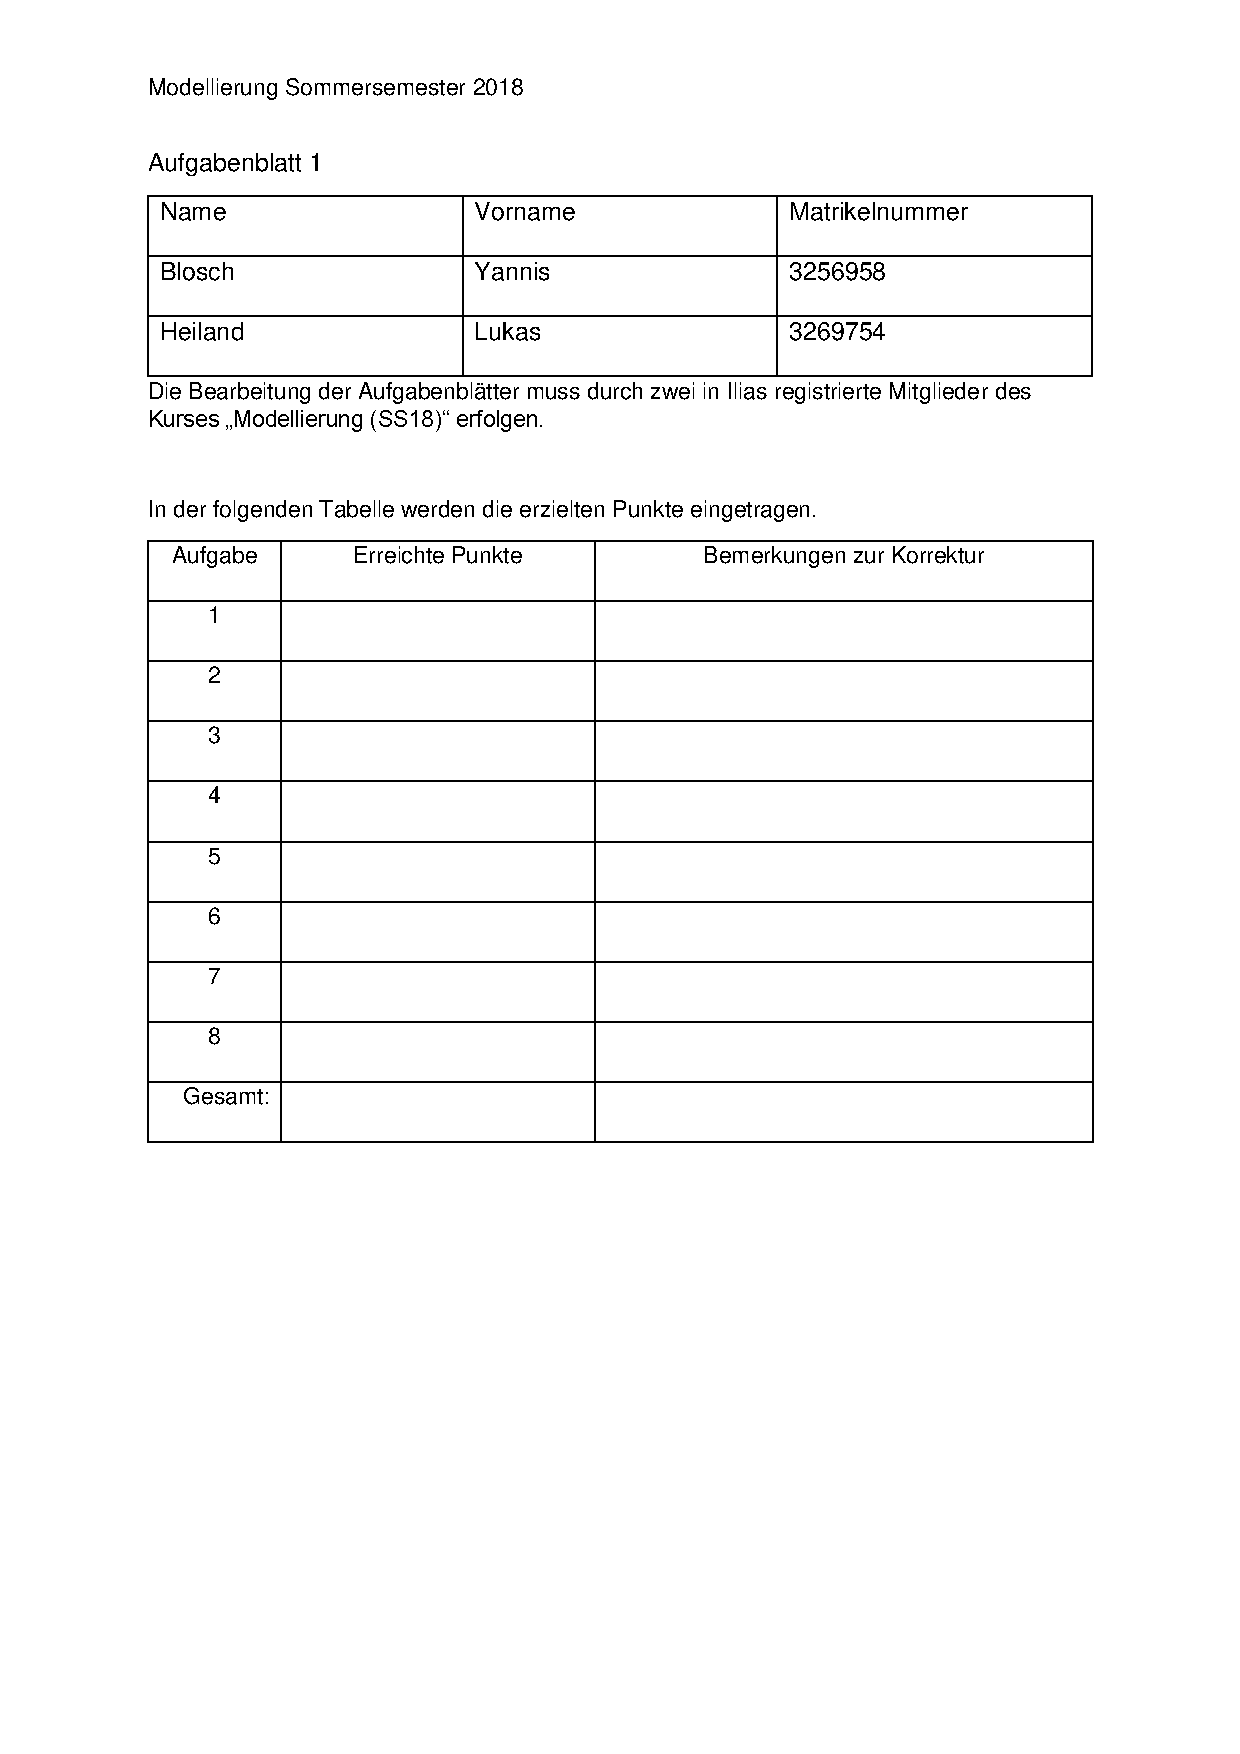
\includepdf{deckblatt.pdf}
	%%% format and header %%%
	% Counter für das Blatt und die Aufgabennummer.
% Ersetze die Nummer des Übungsblattes und die Nummer der Aufgabe
% den Anforderungen entsprechend.
% Beachte:
% \setcounter{countername}{number}: Legt den Wert des Counters fest
% \stepcounter{countername}: Erhöht den Wert des Counters um 1.
\newcounter{sheetnr}
\setcounter{sheetnr}{1} % Nummer des Übungsblattes
\newcounter{exnum}
\setcounter{exnum}{1} % Nummer der Aufgabe

% Befehl für die Aufgabentitel
\newcommand{\exercise}[1]{\section*{Aufgabe \theexnum\stepcounter{exnum} #1}} % Befehl für Aufgabentitel

% Formatierung der Kopfzeile
% \ohead: Setzt rechten Teil der Kopfzeile mit
% Namen und Matrikelnummern aller Bearbeiter
\ohead{Yannis Blosch (3256958)\\
Lukas Heiland (3269754)}
% \chead{} kann mittleren Kopfzeilen Teil sezten
% \ihead: Setzt linken Teil der Kopfzeile mit
% Modulnamen, Semester und Übungsblattnummer
\ihead{Modellierung\\
Sommersemester 2018\\
Blatt \thesheetnr}
	
	\section*{Aufgabe 5.1}
		\paragraph*{a.} Ein Schl"usselkandidat $ \Gamma $ enth"alt alle Attribute, die auf keiner rechten Seite der funktionalen Abh"angigkeiten in $ \mathcal{X} $ stehen. Des weiteren muss f"ur alle Attribute $A \in \mathcal{R} $ gelten: $ A \in (\Gamma)^+ $; dar"uber hinaus muss $ \Gamma $ minimal sein, d.h. es darf keine andere Attributmenge geben, die die vorigen Anforderungen erf"ullt und weniger Elemente enth"alt als $ \Gamma $.\\\\[1.2em] 
		%%%%%%%%%%%%%%%%% 1. CK %%%%%%%%%%%%%%%%
		\textbf{1. Schl"usselkandidat: }$ \mathbf{DL }$\\
		\begin{itemize}
			\item L steht auf keiner rechten Seite, $ L \in DL $ \checkmark
			\item $ (DL)^+: 0. \{D,L\} $\\
			$ 1. \{D,L,E,G,H\} $ \hspace*{20mm}wegen $ DL \rightarrow EGH $\\
			$ 2. \{D,L,E,G,H,J\} $ \hspace*{17mm}wegen $ E \rightarrow J $\\
			$ 3. \{D,L,E,G,H,J,F,K\} $ \hspace*{9mm}wegen $ G \rightarrow FK $\\
			$ \Rightarrow \mathcal{R} \in (DL)^+$ \checkmark
			\item $ DL $ ist minimal (folgt aus Vorbemerkung) \checkmark
		\end{itemize}
		
			
\end{document}